\documentclass[]{article}
\usepackage{caption,subcaption,graphicx,float,url,amsmath,amssymb,amsthm,tocloft,cancel,thmtools,gensymb,braket}
\usepackage[toc,nonumberlist]{glossaries}
\usepackage{glossaries-extra}
\usepackage[toc,page]{appendix}

\newcommand\numberthis{\addtocounter{equation}{1}\tag{\theequation}}

\newtheorem{thm}{Theorem}
\newtheorem{defn}[thm]{Definition}
\newtheorem{cor}[thm]{Corollary}
\newtheorem{lemma}[thm]{Lemma}
\graphicspath{{figs/}}
\widowpenalty10000
\clubpenalty10000
\setcounter{tocdepth}{2}

%opening
\title{Theoretical Minimum\\Particle Physics 2\\Standard Model}
\author{Simon Crase(compiler)}

\begin{document}

\maketitle

\begin{abstract}
These are my notes for the \emph{New Revolutions in Particle Physics 2} lectures from Leonard Susskind's \emph{Theoretical Minimum} series\cite{susskind2009standard}. Since this material predates the discovery of the Higgs Boson, there is an appendix \emph{Demystifying the Higgs Boson} \cite{susskind2010demystifing}.
\end{abstract}

\tableofcontents
\listoffigures
\listoftables
\listoftheorems

\section{Particles fields and forces}

There is a triangle of concepts:
\begin{itemize}
	\item particles (quanta of fundamental fields)\footnote{We are going to have to think very hard about what is an elementary particles and what is composite always be frustrated, always find some slippery region why your definition did not work.}
	\item Fields
	\item Forces
\end{itemize}

\begin{figure}[H]
	\begin{center}
		\caption{Triangle of concepts: particles, fields, and forces}
		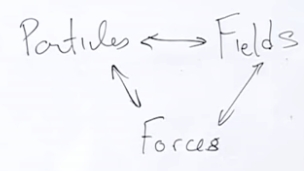
\includegraphics[width=0.5\textwidth]{ParticlesFieldsForces}
	\end{center}
\end{figure}

Consider two electric charges

\begin{align*}
E=&\int (e_1 \vec{E_1})^2 dV\\
E=&\int (e_2 \vec{E_2})^2 dV\\
E=&\int (e_1\vec{E_1}+e_2 \vec{E_2})^2 dV\\
=&\int \underbrace{(e_1\vec{E_1})^2}_\text{self energy}+ \underbrace{(e_2\vec{E_2})^2}_\text{self energy} + \underbrace{2e_1e_2\vec{E_1}.\vec{E_2}}_\text{interesting term}
\end{align*}

The first two terms represent self energy, which is includes in mass; the last term is proportional to the charges.
\begin{itemize}
	\item  If they are so far away that $\vec{E_1}$ is negligible near second charge there will be no perceptible effect.
	\item If the particles are close we will get a contribution from $\vec{E_1}.\vec{E_2}$. This turns out to be the Coulumb force. 
\end{itemize}

The force comes from the distortion of the field: this is a \emph{purely field view of forces}. If fields give rise to forces, and particles are quanta of fields, there must be a way to think of forces coming from particles.

Where do molecular forces come from? There are several mechanisms: we will focus on one. Imagine two protons and a single electron. Electron hops because of tennelling. \footnote{Don't watch tunnelling! Like any QM effect, watching ruins it.}

\begin{figure}[H]
	\caption[Molecular forces: two protons and a single electron]{Two protons and a single electron. Classically electron can't swap between Figures \ref{fig:2proton1Electrona} and \ref{fig:2proton1Electronb}, but QM allows it to tunnel.}
	\begin{subfigure}{0.45\textwidth}
		\caption{Right hand protons is a long way from Left: Schr\"odinger wave function for electron near left hand.} 
		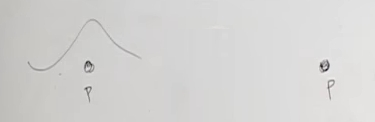
\includegraphics[width=0.9\textwidth]{2proton1Electrona}\label{fig:2proton1Electrona}
	\end{subfigure}
	\begin{subfigure}{0.45\textwidth}
		\caption{Protons closer together: Figure \ref{fig:2proton1Electrona} still possible, but so is this--same energy.}
		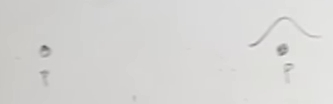
\includegraphics[width=0.9\textwidth]{2proton1Electronb}\label{fig:2proton1Electronb}
	\end{subfigure}
	\begin{subfigure}{0.45\textwidth}
		\caption{Effect of tunnelling}
		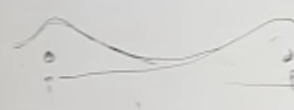
\includegraphics[width=0.9\textwidth]{2proton1Electronab}\label{fig:2proton1Electronab}
	\end{subfigure}
	\begin{subfigure}{0.45\textwidth}
		\caption{Energy as a function of distance between protons. Gradient in energy tries to move protons together, but Coulomb force tries to separate them. Nett effect is a covalent bond.}
		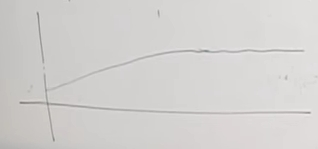
\includegraphics[width=0.9\textwidth]{2proton1ElectronEnergy}\label{fig:2proton1ElectronEnergy}
	\end{subfigure}
	\begin{subfigure}{0.45\textwidth}
		\caption{Electron exchange between protons. This lowers energy, leading to attraction.}
		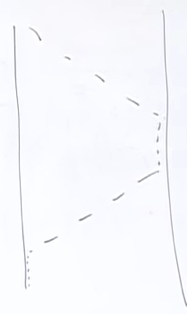
\includegraphics[width=0.9\textwidth]{2proton1ElectronHopping}\label{fig:2proton1ElectronHopping}
	\end{subfigure}
\end{figure}

Key idea: adding wave functions leads to a lower energy state. Energy lowered by alternating between states.

Add 2nd electron, then total charge is zero, giving nett attraction. 

\begin{itemize}
	\item So classically, add 2nd charge, lower energy (creates force) by distorting wave function.
	\item In QM, possibility of swapping between states lowers energy.
\end{itemize}
Can we think of Coulumb force in QM terms? Consider single proton and electron: proton interacts with electromagnetic field, whose quanta are photons.

\begin{itemize}
	\item Classically we solve field equations;
	\item In QM we think of emission and absorption of photons; this is what the Lagrangian tells us. One way to think of this is that the electron is a QM superposition of states: no photons, one with photon emitted,  one with two photons emitted, photon reabsorbed--Figure \ref{fig:2-1-electron-photons}. In Figure \ref{fig:2-1-electron-photons}, when electrons very far apart, energies just add. When they get closer, fields interact, or, in the language of Feynman diagrams, one electron absorbs electron emitted by the other--Figure \ref{fig:2-1-electron-photons-feynmann}.  Energy is no longer sum of energies of individual electrons, which gives rise to Coulomb force.
\end{itemize}

\begin{figure}[H]
	\caption{Emission and absorption of photons}
	\begin{subfigure}{0.45\textwidth}
		\caption{Electron absorbing and reabsorbing photons.}
		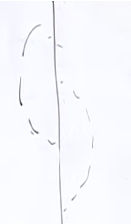
\includegraphics[width=0.9\textwidth]{2-1-electron-photons0}
	\end{subfigure}
	\begin{subfigure}{0.45\textwidth}
		\caption{The electron is a QM superposition of states}\label{fig:2-1-electron-photons}
		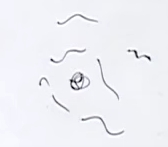
\includegraphics[width=0.9\textwidth]{2-1-electron-photons}
	\end{subfigure}
	\begin{subfigure}{0.45\textwidth}
		\caption{Two Electrons absorbing and reabsorbing photons.}\label{fig:2-1-second-electron-photons}
		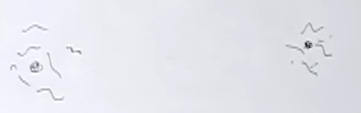
\includegraphics[width=0.9\textwidth]{2-1-second-electron-photons}
	\end{subfigure}
		\begin{subfigure}{0.45\textwidth}
		\caption{Feynman diagram of Electrons absorbing and reabsorbing photons. Sometimes one electron absorbs photon emitted to other.}\label{fig:2-1-electron-photons-feynmann}
		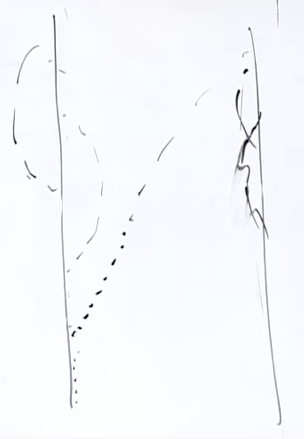
\includegraphics[width=0.9\textwidth]{2-1-second-electron-photons-feynman}
	\end{subfigure}
\end{figure}

In summary we have three ways of looking at forces:

\begin{itemize}
	\item Laws such as Coulomb;
	\item Classical fields theory;
	\item exchange of particles. Every particle can be exchanged, so every particle produces a force. Not just 4 forces! 
\end{itemize}

Standard Model is a mess. We don't understand why the particles are as they are. We understand some relationships. More types of particles than known relationships.

\begin{table}[H]
	\begin{center}
		\caption{Particles (Field symbol)}
		\begin{tabular}{|l|l|l|r|l|r|}\hline
			Name&Symbol&Type&Charge&B\#&Mass\\ \hline
			photon&$\gamma$ A&B&0&0&0 \\ \hline
			electron&$e+\pm \Psi_e\}$&F&-1&0&$0.15MeV$\\ \hline
			Quark&q&F&&$\frac{1}{3}$&\\ \hline
			down&q(Q) $\Psi_q$&F&$-\frac{1}{3}$&$\frac{1}{3}$&10meV\\ \hline
			up&&F&$\frac{2}{3}$&$\frac{1}{3}$&5meV\\ \hline
			strange&&F&$-\frac{1}{3}$&$\frac{1}{3}$&100meV\\ \hline
			charm&&F&$\frac{2}{3}$&$\frac{1}{3}$&1GeV\\ \hline
			bottom&&F&$-\frac{1}{3}$&$\frac{1}{3}$&5Gev\\ \hline
			top&&F&$\frac{2}{3}$&$\frac{1}{3}$&170Gev\\ \hline
			&&&&&\\ \hline
			&&&&&\\ \hline
		\end{tabular}
	\end{center}
\end{table}

\begin{enumerate}
	\item Particle and Field usually have the same name
	\item charge--electron is unit
	\item eV
	\item Proton has Baryon number 1.
	\item 3 families of quarks. Why?
\end{enumerate}

Figure \ref{table:mesons} depicts the way that electromagnetic processes emerge from a Lagrangian.

\begin{figure}[H]
	\caption{$\mathcal{L}$: $e \Psi_e^\dagger \Psi_e A$}\label{fig:fep}
	\begin{subfigure}{0.45\textwidth}
		\caption{Fundamental electromagnetic process. Can rearrange.}
		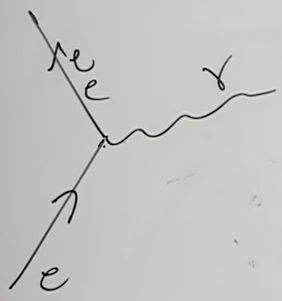
\includegraphics[width=0.9\textwidth]{2-1-em-process}
	\end{subfigure}
	\begin{subfigure}{0.45\textwidth}
		\caption{Fundamental electromagnetic process--exchange of particle.}
		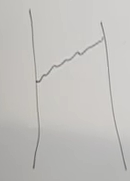
\includegraphics[width=0.9\textwidth]{2-1-em-process-feynman}
	\end{subfigure}
\end{figure}

Three quarks build baryons, two mesons--Table \ref{table:mesons}.
\begin{itemize}
	\item neutron: ddu (slightly heavier)
	\item proton: uud (self energy of energy partially offsets difference in quark masses)
\end{itemize}

Can we make an analogue of proton/neutron with strange quarks? Yes. E.g. sdu, ssu, uus -- Strange baryons.


\begin{table}[H]
	\begin{center}
		\caption[Mesons: baryon number 0 - quark + anti-quark]{Mesons: baryon number 0 - quark + anti-quark. Note the two entangled pairs: $\frac{1}{\sqrt{2}}\big(\ket{\bar{u}u}\pm\ket{\bar{d}d}\big)$}\label{table:mesons}
		\begin{tabular}{|l|l|l|r|} \hline
			&Quarks&Charge&Mass\\ \hline
			$\pi^-$&$\bar{u}d$&-1&$\approx140 meV$ \\ \hline
			$\pi^+$&$u\bar{d}$&+1&$\approx140 meV$  \\ \hline
			$\pi^0$&$\frac{1}{\sqrt{2}}\big(\ket{\bar{u}u}+\ket{\bar{d}d}\big)$&0&$\approx140 meV$  \\ \hline
			$\eta$&$\frac{1}{\sqrt{2}}\big(\ket{\bar{u}u}-\ket{\bar{d}d}\big)$& 0&$\approx500 meV$ \\ \hline
			&$\bar{u}s$&-1& \\ \hline
			&$u\bar{s}$&+1& \\ \hline
			&$\bar{d}s$&0& \\ \hline
			&$d\bar{s}$&0& \\ \hline
			&$\bar{s}s$&0& \\ \hline
		\end{tabular}
	\end{center}
\end{table}

We also have strange mesons ($K-mesans$).


\section{Quantum chromodynamics}

This is the theory of Quarks and gluons, and the things that they make.

\begin{defn}[Hadron]
	The things that Quarks and gluons make are called hadrons.
\end{defn}

\begin{defn}[Baryon]
	Things made from 3 quarks are called baryons.
\end{defn}

\begin{defn}[Meson]
	Mesons are quark-anti-quark pairs.
\end{defn}

\begin{defn}[Gluon]
	Electrically neutral stuff than holds quarks and antiquarks together.
\end{defn}

Spin without group theory. We start with the basic commutation relations:\cite{susskind2009particles}
\begin{align*}
	[L_x,L_y] =& i \hslash L_z\\
	[L_y,L_z] =& i \hslash L_x\\
	[L_z,L_x] =& i \hslash L_y
\end{align*}

In \cite{susskind2009particles}:

\begin{itemize}
	\item We broke the symmetry by focusing on $L_z$.
	\item We can measure only one $L_i$ at a time.
	\item $L_i$ is quantized--$\hslash$.
\end{itemize}

\begin{table}[H]
	\begin{center}
		\caption{Spin multiplets: Spin $l$ denotes highest $L_z$.}
		\begin{tabular}{|c|c|l|} \hline
		$l$&Range of $L_z (Number=2l+1)$&Statistics\\ \hline
		$0$&$0$& Boson\\ \hline
		$\frac{1}{2}$&$\{-\frac{1}{2},\frac{1}{2}\}$& Fermion\\ \hline
		$1$&$\{-1,0,1\}$&Boson \\ \hline
		$\frac{3}{2}$&$\{-\frac{3}{2},-\frac{1}{2},\frac{1}{2},\frac{3}{2}\}$&Fermion \\ \hline
		$2$&$\{-2,-1,0,1,2\}$&Boson \\ \hline
		\end{tabular}
	\end{center}
\end{table}

\begin{table}[H]
	\begin{center}
		\caption[Ways to put two spin $\frac{1}{2}$ particles together]{Ways to put two spin $\frac{1}{2}$ particles together. Consider whether particles could disappera with violating conservation of angular momentum.}
		\begin{tabular}{|l|l|l|l|}\hline
			&$l$&$L_z$&Could disappear?\\ \hline
			$\ket{\uparrow\uparrow}$ &1&1&no--has $L_z$\\ \hline
			$\ket{\downarrow\downarrow}$&1&-1&no--has $L_z$ \\ \hline
			$\frac{1}{\sqrt{2}}(\ket{\uparrow\downarrow}+\ket{\downarrow\uparrow})$ &1&0&no--has $L_x$\\ \hline
			$\frac{1}{\sqrt{2}}(\ket{\uparrow\downarrow}-\ket{\downarrow\uparrow})$ &0&0&yes\\ \hline
		\end{tabular}
	\end{center}
\end{table}

\url{https://youtu.be/yy989li6xgY?t=1171}

\section{Group theory – part 1}



\section{Group theory – part 2}



\section{Gauge fields and symmetry}



\section{The weak interaction}



\section{Spontaneous symmetry breaking and Goldstone bosons}



\section{The Higgs field}






\section{The Higgs field and fermions}



\section{Renormalization and the running of coupling constants}


\begin{appendices}
	\section{Demystifying the Higgs Boson}
	\cite{susskind2010demystifing}
\end{appendices}

\bibliographystyle{unsrt}
\addcontentsline{toc}{section}{Bibliography}
\bibliography{tm}


\end{document}
